\documentclass{article}
\title{MBASE Artificial Intelligence Protocol (MAIP) Version 1.1 First Draft}
\author{Saul Emre Erdoğ}
\usepackage{lipsum}% for some dummy text
\usepackage{fancyhdr}
\usepackage{graphicx}
\usepackage{multirow}
\usepackage{soul}
\date{August 2024}
\pagestyle{fancy}
\renewcommand{\arraystretch}{1.5}
\begin{document}

\maketitle
\fancyfoot{}
\fancyfoot[LO,CE]{\textit{Document Id: MET-MBINF-1-DF1}}
\fancyfoot[LE,RO]{\thepage}
\begin{abstract}
Through the emerge of open-source LLMs and local inference, multiple inference engine solutions have been created.
This created the need for a unified interface for serving the LLMs to public and to allow LLMs to talk to each other for specific tasks.
For that we propose an application-layer, text-based, peer-to-peer MBASE Artificial Intelligence Protocol (MAIP) to serve the functionality of the target inference engine.
What MAIP does in general is that it allows other MAIP programs (Consumer, Producer, C/P) to configure the inference engine through INF calls and executes input through EXEC calls.
The program that serves the engine is called MAIP Producer and the program that uses the engine is called MAIP Consumer and the programs that do both are called MAIP C/P.  
The protocol imposes a standard for the inference engine to served but it is not mentioned in this draft.
\end{abstract}

\begin{center}
\begin{tabular}{  l | p{8cm}  }
\multicolumn{2}{ c }{\textbf{Document Identification}} \\

\textbf{Document name} & MBASE Artificial Intelligence Protocol (MAIP) Version 1.1 First Draft\\
\hline
\textbf{Document ID} & MET-MBINF-1-DF1\\
\hline
\textbf{Authors} & Saul Emre Erdoğ\\
\hline
\textbf{State} & Draft, Active, Unstable, Unfinished\\
\hline
\textbf{Complying Documents} & None \\
\hline
\textbf{Referenced Documents} & None \\
\hline
\end{tabular}
\end{center}

\newpage 
\tableofcontents

\newpage

\section{Introduction}
\subsection{Thoughts on the Current state of AI and LLMs}

In this age, the emergence of AI and its rapid development surely will find a place in the business side. The text-to-text use of LLMs (ChatGPT, Claude etc.) has provided and still provides a lot of benefits to the public. However, there is a difficulty in integrating those public LLMs or locally running LLMs to domain specific applications and programs. In 2024, the system is designed in a way that the single big organization will provide the LLM service with huge data centers and millions of dollars of worth of GPU's running trillion parameter LLM's. Accessing the services provided by big LLMs is a standard for a while which will surely expire. There can be assumed three reasons for that.\newline

The first is the cost and unnecessary use of big LLMs for single and simple tasks. It is estimated that the GPT4.0 has 1 trillion parameters which is expected to be used by the public for all kinds of tasks. It is unfortunate that this huge model is being run to answer questions like "what should I eat today", "summarize this text" etc. The problem is not the questions themselves but invoking that huge model for that. The finely tuned models that is specialized for a specific task with lower parameters like 1.5B or even less, can answer most of the questions people ask to ChatGPT today. 1.5B and 1T are big difference in computing power and optimization.\newline

The second reason is the availability of LLMs. Running big models surely requires a lot of engineering and proper architecture to work well. Not all organizations have the capability to run those LLMs because of the cost and engineering and it is rightly so. Because of this the idea of open-source local LLMs emerged to run locally on your own device. The local LLMs work fine for personal use. However, it seems far away for use in business-applications. The reason for that may be that there is not a consensus on how to serve the AI to the public, undefined standards for serving etc. I claim that the MAIP protocol will fill a hole in this area of thought.\newline

The third reason is confidentiality. This is generally the case for companies. It is clear that the LLMs are so useful for text processing, assisting users daily etc. However, since I have mentioned enough that the companies that serve LLMs are serving these LLMs in their own cloud and computing environment. The companies want to use the LLM but do not want their documents, classified information or anything that is inside to be exposed to the cloud that is far away. Because of this, they prohibit their employees from uploading company documents or using the big LLMs because of the fear of information leak. Through the MAIP protocol and local inference, this problem will surely be overcome.\newline

All in all, local inference has a place in computing and new technologies will emerge in the future, to benefit from it. MAIP protocol is one of those steps to go further for local LLM inference.

\subsection{About MAIP}
MAIP is an application layer text-based protocol that is designed for programs that require high performance and reliable communication with LLM inference engines. Its intended use areas may span from web and mobile applications to low-level embedded systems. For MAIP to be served, a server must have a functioning LLM inference engine that can serve multiple users concurrently.
Even though the protocol does not define the constraints on how to security of the server or inference engine should be handled, it defines how a client session should be managed is defined in client initialization section.\newline

Higher level protocols (OpenAI HTTP etc.) should be implemented in third-party agents that communicate with MAIP server.
\subsection{Requirements}
All documents related to the MBASE Artificial Intelligence Protocol (MAIP) shall use the keywords "MUST", "MUST NOT", "REQUIRED", "SHALL", "SHALL NOT", "SHOULD", "SHOULD NOT", "RECOMMENDED", "MAY", and "OPTIONAL" to describe requirements.\newline

\textbf{Note: }
The structure of this title and conventions are directly inspired and taken from RFC document conventions. Those conventions are described in \underline{RFC 2119}.

\subsection{Syntax Notation}
Since MAIP presents a text interface to communicate, a concrete and well-defined notation should be used to identify the message fields and its syntax. Because of this, this document will use the \textbf{Augmented Backus-Naur Form (ABNF)} to define its syntax.\newline

ABNF is a well-defined syntax notation for defining the syntax of your language or protocol. The ABNF syntax notation is explained and defined with detail in \underline{RFC 5234}. \newline

This document will use the core syntax definitions that are defined in Appendix B.1 of \underline{RFC 5234}. The core definitions used by this document are CR, CRLF, LF, SP, WSP, OCTET, ALPHA, DIGIT and VCHAR.

\section{Overview}
In this section, the overall model of the structure and packet schematic will be shown.
\begin{figure}[h!]
  \centering
  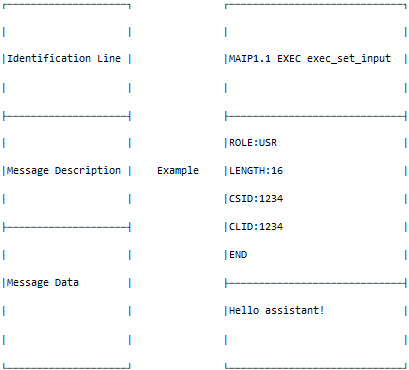
\includegraphics[width=0.7\textwidth]{packet_schematic.png}
  \caption{MAIP Packet Schematic}
\end{figure}

\subsection{Protocol Model}
\begin{figure}[h!]
  \centering
  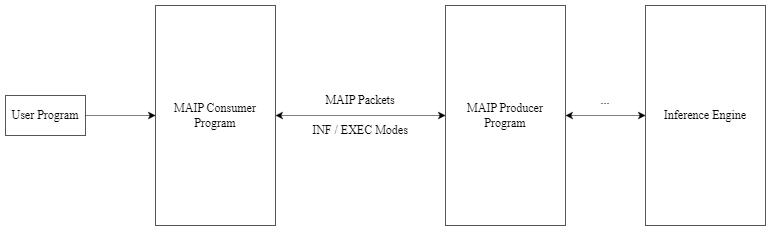
\includegraphics[width=1.2\textwidth]{protocol_model.png}
  \caption{Protocol Model}
\end{figure}
MAIP is a peer-to-peer request/response-based protocol that lifts the inference engine from being isolated to an accessible network layer. The protocol should be thought of as an abstraction layer over the inference engine. Through MAIP, the peer will be able to invoke methods on the target LLM, configure the LLM and the general behavior of the engine etc.\newline

Any program that uses the MAIP protocol can only be at one of these three states such as: Consumer, Producer, Consumer/Producer (CP). Consumer is a program that merely invokes or modifies the inference engine on the target producer. On the other hand, the producer is the one who serves the inference engine to other consumers. If the program is C/P, it will serve as the inference engine and act as a consumer at the same time. \newline

The inference engine will have two modes given as: INF and EXEC modes. The INF mode stands for "information" mode and EXEC mode stands for "execution" mode. \newline

Through INF mode, the consumers will be able to configure the engine, change its state, and other essential operations before executing the user input on the target LLM. On the other hand, the EXEC mode will be used to set the input and execute it on the engine. The operations that are made through INF and EXEC modes are contextual per consumer. In other words, the producer will store a different state for each consumer that is using the inference engine.\newline

For consumers to start using the engine, they MUST go through the client initialization stage which will contextualize the client and disallow unauthorized access (This explained in detail in section999). After the initialization stage is completed, the client will be able to access the services of the engine.\newline
\section{Message Structure}
As section 2 shows the structure of the MAIP packet, this section explains how the message is structured to be delivered to another MAIP program. The MAIP packet is divided into three sections such as identification line, message description, and message data. Among these, only the identification line is different on request and response which will be mentioned now.\newline

\underline{The syntax, constraints and formal definitions are given in section999.}
\subsection{Identification Line}
As the name suggests, the first line of the message identifies the packet itself. It shows whether the message is a request or response, the version of MAIP protocol etc. The messages can only be either request or response message, and this is shown in the identification line as follows. The below is an example request identification line:\newline

\textbf{MAIP1.1 INF inf\_create\_client}\newline

The string until INF is the version indicator of the message which will both be present at the request and response. The INF is called the operation type (OPTYPE) and the \textbf{inf\_create\_client} part is called the operation string (OPSTRING). This OPTYPE \textbf{SHALL} either be \textbf{INF} or \textbf{EXEC} on the protocol. However, different OPTYPEs may be implemented on custom MAIP programs.\newline

The response identification line on the other hand is much simpler. It only contains the version indicator and the response code. The below is an example response identification line:\newline

\textbf{MAIP1.1 2000}\newline

\underline{The description of those response codes is given in their corresponding chapter.}\newline

The syntax is as follows:

\textbf{
\newline
maip-proto-major = 1*4DIGIT\newline
maip-proto-minor = 1*4DIGIT\newline
maip-proto-version-number = maip-proto-major "." maip-proto-minor\newline
maip-proto-name = "MAIP"\newline
maip-version = maip-proto-name maip-proto-version-number\newline
maip-req-op-type = "INF" / "EXEC" / 1*32(VCHAR)\newline
maip-req-op-name = 1*64(VCHAR)\newline
maip-req-op-string = maip-req-op-type SP maip-req-op-name\newline
maip-req-identification-line = maip-version SP maip-req-op-string\newline
maip-resp-status-code = 4*4DIGIT\newline
maip-resp-identification-line  = maip-version SP maip-resp-status-code\newline
maip-identification-line = maip-req-identification-line / maip-resp-identification-line SP LF\newline
}

\subsubsection{Version Mismatch}
In case of MAIP version mismatch between program A and program B, it is up to the user to handle such cases. He can either ignore, depict warning or wholly discard the message. There is no specification on what to do on version mismatch of the message.

\subsection{Message Description}
Message description is a set of key value pairs and an \textbf{"END"} sentence at the end of the description. Those key values describe the message and \textbf{MAY} also be parameters for the specified OPTYPE and OPSTRING. Whether the message is a request or response, does not change the structure of the message description.\newline

Message keys can have either multiple or single values. 	For single keys, the format is simple "key:value" type. However, if multiple values are specified for single key, they \textbf{MUST} either be separated by semicolon ";" character, or there \textbf{MUST} be multiple lines of key value pairs.\newline

As for the latter, if there are multiple lines of same key that correspond to different values, they \textbf{MUST} be parsed in a way that will concatenate all values of the same key. Below is an example of how to have a multiple value for a key: \newline

\begin{figure}[h!]
  \centering
  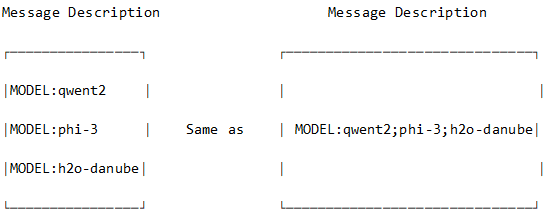
\includegraphics[width=1\textwidth]{multiple_keys.png}
  \caption{Multiple key example}
\end{figure}

The syntax is as follows:\newline
\textbf{
\newline
message-description-key = ALPHA *64(VCHAR)\newline
message-description-value = *256(VCHAR / WSP)\newline
message-description = message-description-key ":" message-description-value *(";" message-description-value) LF\newline
maip-end = "END" LF\newline
}

\subsection{Message Data}
If a LENGTH key/value pair is present in the message description, it shows that the message data is present in the packet. The message data section will contain data whose format, encoding is determined by the key "ENCODING". If the ENCODING key is not present, UTF-8 will be assumed in the data section. \newline

The syntax is as follows:\newline

\textbf{
\newline
message-data = *OCTET
}

\section{Request Modes}
In the previous sections, it is shown that the request can have two modes of execution, it is either INF or EXEC. Through INF requests, the user will authenticate to target machine, acquire model, create new contexts etc. The methods for such operations are named as: \textbf{inf\_create\_session}, \textbf{inf\_acquire\_model}, \textbf{inf\_create\_context} etc. There \textbf{MAY} be many different INF and EXEC operations that will differ with each MAIP protocol version. However, to have a unified structure and to achieve at least basic functionality, there is a minimum constraint of list of operations a MAIP producer \textbf{MUST} support.\newline

The question of how a client is initialized, how an input execution work etc. are mentioned in section overall usage. This section will give only a brief explanation.

\subsection{Inform Request (INF)}
INF request is going to be used to inform the target producer to configure and modify the client according to its needs. For example, to be able to use the functionality that is being served by the producer, the consumer \textbf{MUST} authenticate itself using \textbf{inf\_create\_session} and use the returned client session id (CSID) and client id (CLID) pair to every either INF or EXEC request.\newline

Through this CSID and CLID, user will be able to invoke the services it wants within its own context. For example, for a consumer to use a model on the target machine, the model first MUST be acquired by the consumer through the operation called \textbf{inf\_acquire\_model}. Before acquiring, the user will query the models through \textbf{inf\_get\_program\_models} operation and the producer will return the models that the target inference engine supports. Here is how the \textbf{inf\_get\_program\_models} and \textbf{inf\_acquire\_model} pipeline would look like:\newline

The text inside the boxes is the MAIP packets and the numbers above is the order of request/responses.\newline

\subsection{Execution Request (EXEC)}
After the client is initialized using \textbf{inf\_create\_session} and all other necessary operations are performed (acquiring model, creating context etc.), the consumer is ready to use the LLM engine. Since EXEC operations invoke the inference engine, they are the ones that put a strain on the inference engine.\newline

Execution requests \textbf{MUST} be sent with consumer's context id that is received via \textbf{inf\_create\_context}. The generated context id (CTXID) will be mapped to CSID and CLID so that, every exec request \textbf{MUST} at least be supplied with three parameters given as CSID, CLID, and CTXID.\newline

\subsection{Custom Request}
Custom request is an undefined request type. If the supplied request type can not be interpreted by the target producer, the corresponding response code will be returned. However, the reason it is called custom is that the given custom request type \textbf{MAY} be handled by the target producer. Products that is using the MAIP protocol who has a custom operation type, \textbf{SHOULD} document their operation type and their corresponding operation strings in a proper way.\newline

\section{About Response Codes}
What distinguishes MAIP response is that its response code. The MAIP response code is a 4-digit response code that gives feedback about the requested operation. The response codes are grouped into three categories in which the last digit of the code indicates its group number, and the rest is the code itself.

\subsection{Code Groups}
The response code groups are 1000, 2000, and 3000 response codes which stands for generic codes, inf codes, and exec codes. If there are problems with the MAIP packet such as, undefined OPTYPE, OPSTRING, or the message structure is invalid etc. the response code will be from the generic code group. If the MAIP packet request is INF request, the response code that has been generated is from the inf code group. If the MAIP packet request is EXEC request, the response code that has been generated is from the exec code group. \ul{However, it is possible that the EXEC requests may return response code from inf code group due to problems such as unauthorized access etc}.\newline

\begin{center}
\begin{tabular}{ | l | p{8cm} | }
\multicolumn{2}{ c }{\textbf{Table of Generic Response Codes}} \\
\hline
\textbf{Responde Code} & \textbf{Description}\\
\hline
\textbf{1000} & Generic Success\\
\hline
\textbf{1001} & Undefined operation type\\
\hline
\textbf{1002} & Undefined operation string\\
\hline
\textbf{1003} & Operation type too long\\
\hline
\textbf{1004} & Operation type non-alpha\\
\hline
\textbf{1005} & Operation string too long\\
\hline
\textbf{1006} & Operation string non-printable\\
\hline
\textbf{1007} & Operation timed out\\
\hline
\textbf{1008} & Invalid identification ending\\
\hline
\textbf{1009} & Invalid version major\\
\hline
\textbf{1010} & Invalid protocol\\
\hline
\textbf{1011} & Data length inconsistency\\
\hline
\textbf{1012} & Missing mandatory keys\\
\hline
\textbf{1013} & Missing operation type\\
\hline
\textbf{1014} & Missing key\\
\hline
\textbf{1015} & Missing data\\
\hline
\textbf{1016} & Packet too large\\
\hline
\textbf{1017} & Packet too short\\
\hline
\textbf{1018} & Packet incomplete\\
\hline
\textbf{1019} & Key length too large\\
\hline
\textbf{1020} & Value length too large\\
\hline
\textbf{1021} & Invalid key/value format\\
\hline
\end{tabular}
\end{center}

\begin{center}
\begin{tabular}{ | l | p{8cm} | }
\multicolumn{2}{ c }{\textbf{Table of Inform Response Codes}} \\
\hline
\textbf{Responde Code} & \textbf{Description}\\
\hline
\textbf{2000} & Inform Success\\
\hline
\textbf{2001} & Client limit reached\\
\hline
\textbf{2002} & Client ID mismatch\\
\hline
\textbf{2003} & Unauthorized access\\
\hline
\textbf{2004} & Model name mismatch\\
\hline
\textbf{2005} & Context ID mismatch\\
\hline
\textbf{2006} & Context limit reached\\
\hline
\textbf{2007} & Unable to find a suitable processor\\
\hline
\textbf{2008} & Unknown status\\
\hline
\textbf{2009} & Client unregistering\\
\hline
\textbf{2010} & Client is not registered\\
\hline
\textbf{2011} & Processor unavailable\\
\hline
\textbf{2012} & Context is active\\
\hline
\textbf{2013} & Context is inactive\\
\hline

\end{tabular}
\end{center}

\begin{center}
\begin{tabular}{ | l | p{8cm} | }
\multicolumn{2}{ c }{\textbf{Table of Exec Response Codes}} \\
\hline
\textbf{Responde Code} & \textbf{Description}\\
\hline
\textbf{3000} & Execution success\\
\hline
\textbf{3001} & Processing\\
\hline
\textbf{3002} & Message id mismatch\\
\hline
\textbf{3003} & Missing message\\
\hline
\textbf{3004} & Tokenization failed\\
\hline
\textbf{3005} & Token limit exceeded\\
\hline
\textbf{3006} & Message continue\\
\hline
\textbf{3007} & Message finished\\
\hline
\textbf{3008} & Context abandoned\\
\hline
\textbf{3009} & Context inactive\\
\hline
\end{tabular}
\end{center}

\section{Overall Usage}
Finally, in this section I will show how to use the MAIP producer to produce output from the desired LLM. For the desired operation to occur, the client \textbf{MUST} initialize itself on the target producer if the CSID and CLID do not exist. If they exist, the client initialization step can be ignored. The steps to use the inference engine are most generally as follows:\newline

\begin{enumerate}
  \item Client initialization.
  \item Querying and acquiring the model.
  \item Creating context.
  \item Setting up input.
  \item Executing the input and obtaining the result.
  \item Cleaning up.
\end{enumerate}

\subsection{Client Initialization}
If the client does not have a CSID and CLID received from the producer before, it \textbf{MUST} first get the CSID and CLID from the producer. Through those keys, client will be authorized to operate on target producer. Along with authorization, it will also contextualize the client in a way that the further operations that are made by the client will only happen in the context of the given client only.\newline

For client to be authorized on the producer, it \textbf{MUST} call the \textbf{inf\_create\_session} operation and receive CSID and CLID from the producer. This CSID and CLID \textbf{MAY} be used by the client if the producer accepts those CSID and CLID pair authoritatively. If in any way, the producer returns response code 2003, it means that the CSID and CLID are expired, and the new ones \textbf{MUST} be acquired from the producer using the same method.\newline

Here is how the MAIP request and response looks like for this operation:\newline

\begin{center}
\begin{tabular}{ | l | p{8cm} | }
\multicolumn{2}{ c }{\textbf{Client Initialization Example}} \\
\hline
\textbf{MAIP Request} & \textbf{MAIP Response}\\
\hline
MAIP1.0 INF inf\_create\_session & MAIP1.0 2000\\
END & CSID: 1234\\
\phantom{invis} & CLID: 1234\\
\phantom{invis} & END\\
\hline
\end{tabular}
\end{center}

\ul{\textbf{After having the CSID and CLID, they MUST be included with every MAIP request, otherwise, unauthorized access (2003) will return as a response code.}}

\subsection{Querying and Acquiring the Model}
The producer \textbf{MAY} host either single or multiple models at the same time. Consumer can get the names of the models that are hosted by producer by invoking the operation inf\_get\_program\_models. Here is how the MAIP request and response looks like for this operation:

\begin{center}
\begin{tabular}{ | l | p{8cm} | }
\multicolumn{2}{ c }{\textbf{Query Model Example}} \\
\hline
\textbf{MAIP Request} & \textbf{MAIP Response}\\
\hline
MAIP1.0 INF inf\_get\_program\_models & MAIP1.0 2000\\
CSID: 1234 & MODEL: qwen2-7b-instruct;phi-3.5;llama3-8b\\
CLID: 1234 & END\\
END & \phantom{invis}\\
\hline
\end{tabular}
\end{center}
After receiving the names of the models that the producer supports, the model \textbf{MUST} be acquired by the client to operate upon. Once the model is acquired, as long as its not released or the client CSID and CLID not being released by the producer, it does not need to be reacquired. However, if the consumer tries to acquire a model that has already been acquired, the producer will be aware of that and ignore the request and just return 2000 success. Here is how the MAIP request and response looks like for this operation:

\begin{center}
\begin{tabular}{ | l | p{8cm} | }
\multicolumn{2}{ c }{\textbf{Acquire Model Example}} \\
\hline
\textbf{MAIP Request} & \textbf{MAIP Response}\\
\hline
MAIP1.0 INF inf\_acquire\_model & MAIP1.0 2000\\
CSID: 1234 & END\\
CLID: 1234 & \phantom{invis}\\
MODEL: phi-3.5 & \phantom{invis}\\
END & \phantom{invis}\\
\hline
\end{tabular}
\end{center}

\subsection{Creating Context}
The last thing to setup before using the inference engine is the creation of the context. Context is like a chat session in popular LLMs (ChatGPT, Claude etc.). The reason it is called a context but not chat is that basically you only chat with text-to-x models, and other models have different types of input/output scenarios. For our case, we are creating a context for text-to-text model. 


\end{document}